%--------------------
% Packages
% -------------------
\documentclass[11pt,english]{article}
\usepackage{amsfonts}
\usepackage[left=2.5cm,top=2cm,right=2.5cm,bottom=3cm,bindingoffset=0cm]{geometry}
\usepackage{amsmath, amsthm, amssymb}
\usepackage{tikz}
\usetikzlibrary{calc}
\usetikzlibrary{decorations.pathreplacing,calligraphy}
\usepackage{fancyhdr}
%\usepackage{currfile}
\usepackage{nicefrac}
\usepackage{cite}
\usepackage{graphicx}
\usepackage{caption}
\usepackage{longtable}
\usepackage{rotating}
\usepackage{lscape}
\usepackage{booktabs}
\usepackage{float}
\usepackage{placeins}
\usepackage{setspace}
\usepackage[font=itshape]{quoting}
\onehalfspacing
\usepackage{mathrsfs}
\usepackage{tcolorbox}
\usepackage{xcolor}
\usepackage{subcaption}
\usepackage{float}
\usepackage[multiple]{footmisc}
\usepackage[T1]{fontenc}
\usepackage[sc]{mathpazo}
\usepackage{listings}
\usepackage{longtable}
\definecolor{cmured}{RGB}{175,30,45}
\definecolor{macroblue}{RGB}{56,108,176}
\usepackage[format=plain,
            labelfont=bf,
            textfont=]{caption}
\usepackage[colorlinks=true,citecolor=macroblue,linkcolor=macroblue,urlcolor=macroblue]{hyperref}
\usepackage{varioref}
\usepackage{chngcntr}
\usepackage{datetime}

\definecolor{darkgreen}{RGB}{30,175,88}
\definecolor{darkblue}{RGB}{30,118,175}
\definecolor{maroon}{rgb}{0.66,0,0}
\definecolor{darkgreen}{rgb}{0,0.69,0}

%Counters
\newtheorem{theorem}{Theorem}[section] 
\newtheorem{proposition}{Proposition}
\newtheorem{lemma}{Lemma}
\newtheorem{corollary}{Corollary}
\newtheorem{assumption}{Assumption}
\newtheorem{axiom}{Axiom}
\newtheorem{case}{Case}
\newtheorem{claim}{Claim}
\newtheorem{condition}{Condition}
\newtheorem{definition}{Definition}
\newtheorem{example}{Example}
\newtheorem{notation}{Notation}
\newtheorem{remark}{Remark}


\hypersetup{ 	
pdfsubject = {},
pdftitle = {TidyTuesday Week 40},
pdfauthor = {Pranay Gundam},
linkcolor= macroblue
}


\title{\textbf{TidyTuesday Week 40}}
\author{Pranay Gundam}


%-----------------------
% Begin document
%-----------------------
\begin{document}

\maketitle

\tableofcontents

\section{Weekly Summary}


\section{Date: 2024-09-30}
\noindent \textbf{Series ID: PRIICLAIMS} 

\noindent This series is titled Initial Claims in Puerto Rico and has a frequency of Weekly, Ending Saturday. The units are Number and the seasonal adjustment is Not Seasonally Adjusted.The observation start date is 1986-02-15 and the observation end date is 2024-09-21.The popularity of this series is 5. \\ 

\noindent \textbf{Series ID: WPU321101} 

\noindent This series is titled Producer Price Index by Commodity: Warehousing, Storage, and Related Services and has a frequency of Monthly. The units are Index Dec 2008=100 and the seasonal adjustment is Not Seasonally Adjusted.The observation start date is 2008-12-01 and the observation end date is 2024-08-01.The popularity of this series is 1. \\ 

\subsection{\subsection{Regression Tables and Plots}}
\begin{center}
\begin{tabular}{lclc}
\toprule
\textbf{Dep. Variable:}          & value\_fred\_WPU321101 & \textbf{  R-squared:         } &     0.028   \\
\textbf{Model:}                  &          OLS           & \textbf{  Adj. R-squared:    } &    -0.014   \\
\textbf{Method:}                 &     Least Squares      & \textbf{  F-statistic:       } &    0.6714   \\
\textbf{Date:}                   &    Mon, 30 Sep 2024    & \textbf{  Prob (F-statistic):} &    0.421    \\
\textbf{Time:}                   &        09:26:38        & \textbf{  Log-Likelihood:    } &   -101.43   \\
\textbf{No. Observations:}       &             25         & \textbf{  AIC:               } &     206.9   \\
\textbf{Df Residuals:}           &             23         & \textbf{  BIC:               } &     209.3   \\
\textbf{Df Model:}               &              1         & \textbf{                     } &             \\
\textbf{Covariance Type:}        &       nonrobust        & \textbf{                     } &             \\
\bottomrule
\end{tabular}
\begin{tabular}{lcccccc}
                                 & \textbf{coef} & \textbf{std err} & \textbf{t} & \textbf{P$> |$t$|$} & \textbf{[0.025} & \textbf{0.975]}  \\
\midrule
\textbf{const}                   &     113.9020  &        7.173     &    15.880  &         0.000        &       99.064    &      128.740     \\
\textbf{value\_fred\_PRIICLAIMS} &      -0.0026  &        0.003     &    -0.819  &         0.421        &       -0.009    &        0.004     \\
\bottomrule
\end{tabular}
\begin{tabular}{lclc}
\textbf{Omnibus:}       &  9.006 & \textbf{  Durbin-Watson:     } &    0.100  \\
\textbf{Prob(Omnibus):} &  0.011 & \textbf{  Jarque-Bera (JB):  } &    7.958  \\
\textbf{Skew:}          &  1.374 & \textbf{  Prob(JB):          } &   0.0187  \\
\textbf{Kurtosis:}      &  3.295 & \textbf{  Cond. No.          } & 5.66e+03  \\
\bottomrule
\end{tabular}
%\caption{OLS Regression Results}
\end{center}

Notes: \newline
 [1] Standard Errors assume that the covariance matrix of the errors is correctly specified. \newline
 [2] The condition number is large, 5.66e+03. This might indicate that there are \newline
 strong multicollinearity or other numerical problems.

\begin{figure}
\centering
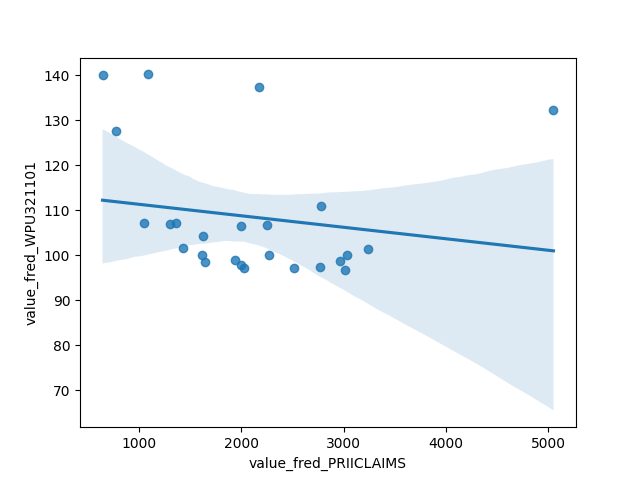
\includegraphics[scale = 0.9]{plots/plot_2024-09-30.png}
\caption{Regression Plot for 2024-09-30}
\end{figure}
\newpage

\section{Date: 2024-10-01}
\noindent \textbf{Series ID: BSCICP035AM665S} 

\noindent This series is titled Composite Leading Indicators: Composite Business Confidence Amplitude Adjusted for Major Five Asia Economies and has a frequency of Monthly. The units are Normalised (Normal=100) and the seasonal adjustment is Seasonally Adjusted.The observation start date is 2000-02-01 and the observation end date is 2023-12-01.The popularity of this series is 4. \\ 

\noindent \textbf{Series ID: CCDIOANYQ156N} 

\noindent This series is titled CredAbility Consumer Distress Index for New York (DISCONTINUED) and has a frequency of Quarterly. The units are Percent and the seasonal adjustment is Not Seasonally Adjusted.The observation start date is 1980-01-01 and the observation end date is 2013-01-01.The popularity of this series is 1. \\ 

\subsection{\subsection{Regression Tables and Plots}}
\begin{center}
\begin{tabular}{lclc}
\toprule
\textbf{Dep. Variable:}               & value\_fred\_CCDIOANYQ156N & \textbf{  R-squared:         } &     0.176   \\
\textbf{Model:}                       &            OLS             & \textbf{  Adj. R-squared:    } &     0.159   \\
\textbf{Method:}                      &       Least Squares        & \textbf{  F-statistic:       } &     10.66   \\
\textbf{Date:}                        &      Tue, 01 Oct 2024      & \textbf{  Prob (F-statistic):} &  0.00198    \\
\textbf{Time:}                        &          14:58:10          & \textbf{  Log-Likelihood:    } &   -154.57   \\
\textbf{No. Observations:}            &               52           & \textbf{  AIC:               } &     313.1   \\
\textbf{Df Residuals:}                &               50           & \textbf{  BIC:               } &     317.0   \\
\textbf{Df Model:}                    &                1           & \textbf{                     } &             \\
\textbf{Covariance Type:}             &         nonrobust          & \textbf{                     } &             \\
\bottomrule
\end{tabular}
\begin{tabular}{lcccccc}
                                      & \textbf{coef} & \textbf{std err} & \textbf{t} & \textbf{P$> |$t$|$} & \textbf{[0.025} & \textbf{0.975]}  \\
\midrule
\textbf{const}                        &     -68.2822  &       44.847     &    -1.523  &         0.134        &     -158.360    &       21.796     \\
\textbf{value\_fred\_BSCICP035AM665S} &       1.4562  &        0.446     &     3.265  &         0.002        &        0.560    &        2.352     \\
\bottomrule
\end{tabular}
\begin{tabular}{lclc}
\textbf{Omnibus:}       &  1.626 & \textbf{  Durbin-Watson:     } &    0.180  \\
\textbf{Prob(Omnibus):} &  0.444 & \textbf{  Jarque-Bera (JB):  } &    1.406  \\
\textbf{Skew:}          & -0.248 & \textbf{  Prob(JB):          } &    0.495  \\
\textbf{Kurtosis:}      &  2.366 & \textbf{  Cond. No.          } & 6.74e+03  \\
\bottomrule
\end{tabular}
%\caption{OLS Regression Results}
\end{center}

Notes: \newline
 [1] Standard Errors assume that the covariance matrix of the errors is correctly specified. \newline
 [2] The condition number is large, 6.74e+03. This might indicate that there are \newline
 strong multicollinearity or other numerical problems.

\begin{figure}
\centering
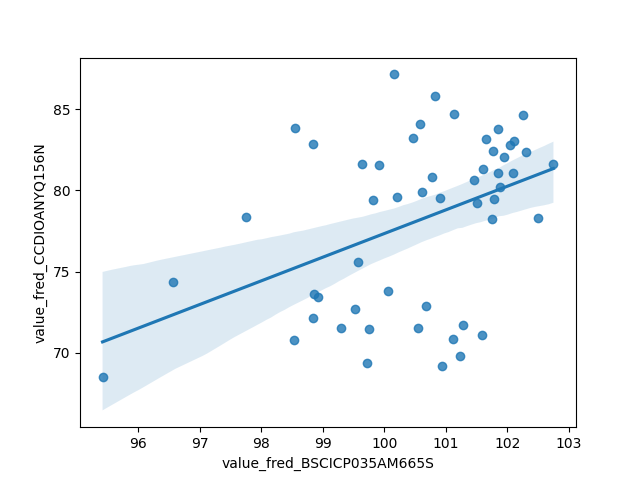
\includegraphics[scale = 0.9]{plots/plot_2024-10-01.png}
\caption{Regression Plot for 2024-10-01}
\end{figure}
\newpage

\section{Date: 2024-10-02}
\noindent \textbf{Series ID: MPCV04XXS} 

\noindent This series is titled Total Private Construction Spending: Health Care in the United States and has a frequency of Monthly. The units are Percent Change from Preceding Period and the seasonal adjustment is Seasonally Adjusted.The observation start date is 2002-02-01 and the observation end date is 2024-08-01.The popularity of this series is 5. \\ 

\noindent \textbf{Series ID: BOPXM} 

\noindent This series is titled Exports of Merchandise: Adjusted, Excluding Military (DISCONTINUED) and has a frequency of Quarterly. The units are Billions of Dollars and the seasonal adjustment is Seasonally Adjusted.The observation start date is 1960-01-01 and the observation end date is 2014-01-01.The popularity of this series is 1. \\ 

\subsection{\subsection{Regression Tables and Plots}}
\begin{center}
\begin{tabular}{lclc}
\toprule
\textbf{Dep. Variable:}         & value\_fred\_BOPXM & \textbf{  R-squared:         } &     0.004   \\
\textbf{Model:}                 &        OLS         & \textbf{  Adj. R-squared:    } &    -0.017   \\
\textbf{Method:}                &   Least Squares    & \textbf{  F-statistic:       } &    0.1986   \\
\textbf{Date:}                  &  Wed, 02 Oct 2024  & \textbf{  Prob (F-statistic):} &    0.658    \\
\textbf{Time:}                  &      13:58:20      & \textbf{  Log-Likelihood:    } &   -275.87   \\
\textbf{No. Observations:}      &           48       & \textbf{  AIC:               } &     555.7   \\
\textbf{Df Residuals:}          &           46       & \textbf{  BIC:               } &     559.5   \\
\textbf{Df Model:}              &            1       & \textbf{                     } &             \\
\textbf{Covariance Type:}       &     nonrobust      & \textbf{                     } &             \\
\bottomrule
\end{tabular}
\begin{tabular}{lcccccc}
                                & \textbf{coef} & \textbf{std err} & \textbf{t} & \textbf{P$> |$t$|$} & \textbf{[0.025} & \textbf{0.975]}  \\
\midrule
\textbf{const}                  &     290.1043  &       11.193     &    25.919  &         0.000        &      267.575    &      312.634     \\
\textbf{value\_fred\_MPCV04XXS} &       2.0497  &        4.599     &     0.446  &         0.658        &       -7.208    &       11.307     \\
\bottomrule
\end{tabular}
\begin{tabular}{lclc}
\textbf{Omnibus:}       & 17.228 & \textbf{  Durbin-Watson:     } &    0.036  \\
\textbf{Prob(Omnibus):} &  0.000 & \textbf{  Jarque-Bera (JB):  } &    3.442  \\
\textbf{Skew:}          & -0.003 & \textbf{  Prob(JB):          } &    0.179  \\
\textbf{Kurtosis:}      &  1.688 & \textbf{  Cond. No.          } &     2.44  \\
\bottomrule
\end{tabular}
%\caption{OLS Regression Results}
\end{center}

Notes: \newline
 [1] Standard Errors assume that the covariance matrix of the errors is correctly specified.

\begin{figure}
\centering
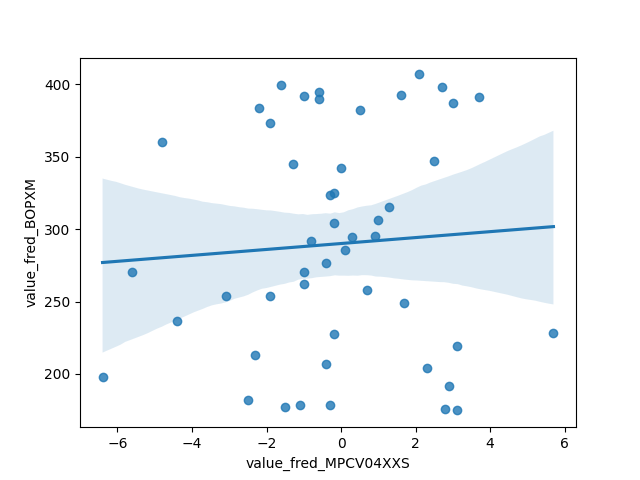
\includegraphics[scale = 0.9]{plots/plot_2024-10-02.png}
\caption{Regression Plot for 2024-10-02}
\end{figure}
\newpage

\section{Date: 2024-10-03}
\noindent \textbf{Series ID: MORTMRGN1SW} 

\noindent This series is titled Margin for 1-Year Adjustable Rate Mortgage in the Southwest Freddie Mac Region (DISCONTINUED) and has a frequency of Weekly, Ending Thursday. The units are Percent and the seasonal adjustment is Not Seasonally Adjusted.The observation start date is 1988-02-19 and the observation end date is 2015-12-31.The popularity of this series is 1. \\ 

\noindent \textbf{Series ID: DHIDFHRVIWTU} 

\noindent This series is titled DHI-DFH Index of Recruiting Intensity per Vacancy by Industry: Warehouse, Trans. & Utilities (DISCONTINUED) and has a frequency of Monthly. The units are Index and the seasonal adjustment is Not Seasonally Adjusted.The observation start date is 2001-01-01 and the observation end date is 2018-04-01.The popularity of this series is 0. \\ 

\subsection{\subsection{Regression Tables and Plots}}
\begin{center}
\begin{tabular}{lclc}
\toprule
\textbf{Dep. Variable:}           & value\_fred\_DHIDFHRVIWTU & \textbf{  R-squared:         } &     0.054   \\
\textbf{Model:}                   &            OLS            & \textbf{  Adj. R-squared:    } &     0.011   \\
\textbf{Method:}                  &       Least Squares       & \textbf{  F-statistic:       } &     1.257   \\
\textbf{Date:}                    &      Thu, 03 Oct 2024     & \textbf{  Prob (F-statistic):} &    0.274    \\
\textbf{Time:}                    &          12:34:14         & \textbf{  Log-Likelihood:    } &    22.287   \\
\textbf{No. Observations:}        &               24          & \textbf{  AIC:               } &    -40.57   \\
\textbf{Df Residuals:}            &               22          & \textbf{  BIC:               } &    -38.22   \\
\textbf{Df Model:}                &                1          & \textbf{                     } &             \\
\textbf{Covariance Type:}         &         nonrobust         & \textbf{                     } &             \\
\bottomrule
\end{tabular}
\begin{tabular}{lcccccc}
                                  & \textbf{coef} & \textbf{std err} & \textbf{t} & \textbf{P$> |$t$|$} & \textbf{[0.025} & \textbf{0.975]}  \\
\midrule
\textbf{const}                    &       3.3356  &        2.073     &     1.609  &         0.122        &       -0.963    &        7.635     \\
\textbf{value\_fred\_MORTMRGN1SW} &      -0.8370  &        0.746     &    -1.121  &         0.274        &       -2.385    &        0.711     \\
\bottomrule
\end{tabular}
\begin{tabular}{lclc}
\textbf{Omnibus:}       &  0.563 & \textbf{  Durbin-Watson:     } &    0.601  \\
\textbf{Prob(Omnibus):} &  0.755 & \textbf{  Jarque-Bera (JB):  } &    0.529  \\
\textbf{Skew:}          &  0.315 & \textbf{  Prob(JB):          } &    0.768  \\
\textbf{Kurtosis:}      &  2.637 & \textbf{  Cond. No.          } &     319.  \\
\bottomrule
\end{tabular}
%\caption{OLS Regression Results}
\end{center}

Notes: \newline
 [1] Standard Errors assume that the covariance matrix of the errors is correctly specified.

\begin{figure}
\centering
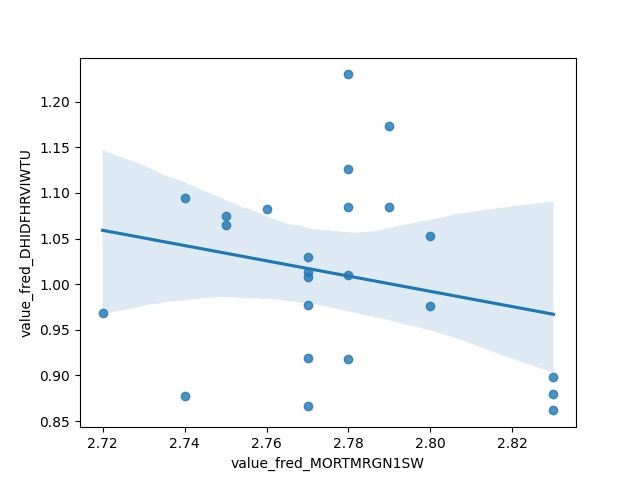
\includegraphics[scale = 0.9]{plots/plot_2024-10-03.png}
\caption{Regression Plot for 2024-10-03}
\end{figure}
\newpage

\section{Date: 2024-10-04}
\noindent \textbf{Series ID: DTRNSNM} 

\noindent This series is titled One to Four Family Real Estate Loans Securitized by Finance Companies, Level and has a frequency of Monthly. The units are Millions of Dollars and the seasonal adjustment is Not Seasonally Adjusted.The observation start date is 1996-06-01 and the observation end date is 2024-07-01.The popularity of this series is 1. \\ 

\noindent \textbf{Series ID: LNU02026623} 

\noindent This series is titled Multiple Jobholders, Women and has a frequency of Monthly. The units are Thousands of Persons and the seasonal adjustment is Not Seasonally Adjusted.The observation start date is 1994-01-01 and the observation end date is 2024-09-01.The popularity of this series is 6. \\ 

\subsection{Regression Tables and Plots}
\begin{center}
\begin{tabular}{lclc}
\toprule
\textbf{Dep. Variable:}       & value\_fred\_LNU02026623 & \textbf{  R-squared:         } &     0.089   \\
\textbf{Model:}               &           OLS            & \textbf{  Adj. R-squared:    } &     0.087   \\
\textbf{Method:}              &      Least Squares       & \textbf{  F-statistic:       } &     32.97   \\
\textbf{Date:}                &     Fri, 04 Oct 2024     & \textbf{  Prob (F-statistic):} &  2.10e-08   \\
\textbf{Time:}                &         11:32:04         & \textbf{  Log-Likelihood:    } &   -2345.0   \\
\textbf{No. Observations:}    &             338          & \textbf{  AIC:               } &     4694.   \\
\textbf{Df Residuals:}        &             336          & \textbf{  BIC:               } &     4702.   \\
\textbf{Df Model:}            &               1          & \textbf{                     } &             \\
\textbf{Covariance Type:}     &        nonrobust         & \textbf{                     } &             \\
\bottomrule
\end{tabular}
\begin{tabular}{lcccccc}
                              & \textbf{coef} & \textbf{std err} & \textbf{t} & \textbf{P$> |$t$|$} & \textbf{[0.025} & \textbf{0.975]}  \\
\midrule
\textbf{const}                &    3783.4423  &       17.699     &   213.765  &         0.000        &     3748.627    &     3818.257     \\
\textbf{value\_fred\_DTRNSNM} &      -0.0044  &        0.001     &    -5.742  &         0.000        &       -0.006    &       -0.003     \\
\bottomrule
\end{tabular}
\begin{tabular}{lclc}
\textbf{Omnibus:}       & 15.893 & \textbf{  Durbin-Watson:     } &    0.456  \\
\textbf{Prob(Omnibus):} &  0.000 & \textbf{  Jarque-Bera (JB):  } &   40.526  \\
\textbf{Skew:}          & -0.014 & \textbf{  Prob(JB):          } & 1.58e-09  \\
\textbf{Kurtosis:}      &  4.696 & \textbf{  Cond. No.          } & 3.01e+04  \\
\bottomrule
\end{tabular}
%\caption{OLS Regression Results}
\end{center}

Notes: \newline
 [1] Standard Errors assume that the covariance matrix of the errors is correctly specified. \newline
 [2] The condition number is large, 3.01e+04. This might indicate that there are \newline
 strong multicollinearity or other numerical problems.

\begin{figure}
\centering
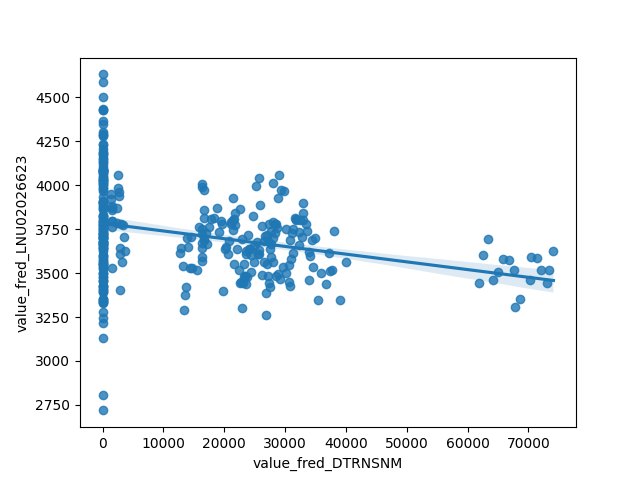
\includegraphics[scale = 0.9]{plots/plot_2024-10-04.png}
\caption{Regression Plot for 2024-10-04}
\end{figure}
\newpage

\section{Date: 2024-10-05}
\noindent \textbf{Series ID: CIS2023211000000I} 

\noindent This series is titled Employment Cost Index: Wages and salaries for Private industry workers in Aircraft manufacturing and has a frequency of Quarterly. The units are Index Dec 2005=100 and the seasonal adjustment is Seasonally Adjusted.The observation start date is 2003-01-01 and the observation end date is 2024-04-01.The popularity of this series is 12. \\ 

\noindent \textbf{Series ID: WHLSLRSMNSA} 

\noindent This series is titled Merchant Wholesalers Sales and has a frequency of Monthly. The units are Millions of Dollars and the seasonal adjustment is Not Seasonally Adjusted.The observation start date is 1992-01-01 and the observation end date is 2024-07-01.The popularity of this series is 4. \\ 

\subsection{Regression Tables and Plots}
\begin{center}
\begin{tabular}{lclc}
\toprule
\textbf{Dep. Variable:}                 & value\_fred\_WHLSLRSMNSA & \textbf{  R-squared:         } &     0.882   \\
\textbf{Model:}                         &           OLS            & \textbf{  Adj. R-squared:    } &     0.881   \\
\textbf{Method:}                        &      Least Squares       & \textbf{  F-statistic:       } &     628.4   \\
\textbf{Date:}                          &     Sat, 05 Oct 2024     & \textbf{  Prob (F-statistic):} &  9.35e-41   \\
\textbf{Time:}                          &         12:30:01         & \textbf{  Log-Likelihood:    } &   -1032.8   \\
\textbf{No. Observations:}              &              86          & \textbf{  AIC:               } &     2070.   \\
\textbf{Df Residuals:}                  &              84          & \textbf{  BIC:               } &     2075.   \\
\textbf{Df Model:}                      &               1          & \textbf{                     } &             \\
\textbf{Covariance Type:}               &        nonrobust         & \textbf{                     } &             \\
\bottomrule
\end{tabular}
\begin{tabular}{lcccccc}
                                        & \textbf{coef} & \textbf{std err} & \textbf{t} & \textbf{P$> |$t$|$} & \textbf{[0.025} & \textbf{0.975]}  \\
\midrule
\textbf{const}                          &   -2.363e+05  &     2.71e+04     &    -8.724  &         0.000        &     -2.9e+05    &    -1.82e+05     \\
\textbf{value\_fred\_CIS2023211000000I} &    5336.9804  &      212.904     &    25.068  &         0.000        &     4913.597    &     5760.364     \\
\bottomrule
\end{tabular}
\begin{tabular}{lclc}
\textbf{Omnibus:}       &  4.890 & \textbf{  Durbin-Watson:     } &    0.918  \\
\textbf{Prob(Omnibus):} &  0.087 & \textbf{  Jarque-Bera (JB):  } &    4.435  \\
\textbf{Skew:}          & -0.381 & \textbf{  Prob(JB):          } &    0.109  \\
\textbf{Kurtosis:}      &  3.811 & \textbf{  Cond. No.          } &     794.  \\
\bottomrule
\end{tabular}
%\caption{OLS Regression Results}
\end{center}

Notes: \newline
 [1] Standard Errors assume that the covariance matrix of the errors is correctly specified.

\begin{figure}
\centering
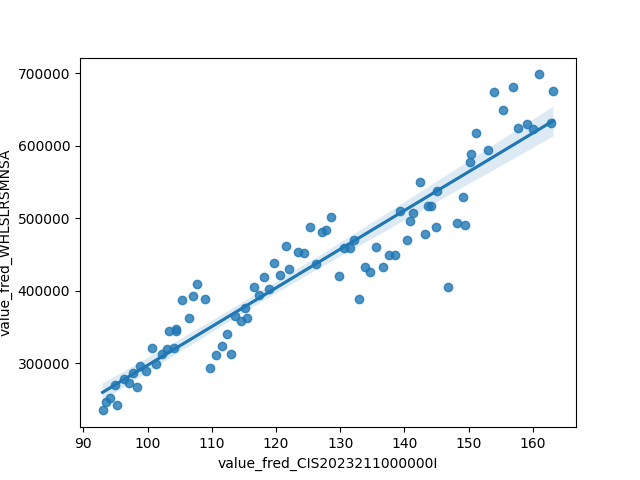
\includegraphics[scale = 0.9]{plots/plot_2024-10-05.png}
\caption{Regression Plot for 2024-10-05}
\end{figure}
\newpage

\section{Date: 2024-10-06}
\noindent \textbf{Series ID: CUURD000SAEC} 

\noindent This series is titled Consumer Price Index for All Urban Consumers: Education and Communication Commodities in Size Class D (DISCONTINUED) and has a frequency of Monthly. The units are Index Dec 2009=100 and the seasonal adjustment is Not Seasonally Adjusted.The observation start date is 2009-12-01 and the observation end date is 2017-12-01.The popularity of this series is 1. \\ 

\noindent \textbf{Series ID: CBBTCUSD} 

\noindent This series is titled Coinbase Bitcoin and has a frequency of Daily, 7-Day. The units are U.S. Dollars and the seasonal adjustment is Not Seasonally Adjusted.The observation start date is 2014-12-01 and the observation end date is 2024-10-05.The popularity of this series is 63. \\ 

\subsection{Regression Tables and Plots}
\begin{center}
\begin{tabular}{lclc}
\toprule
\textbf{Dep. Variable:}            & value\_fred\_CBBTCUSD & \textbf{  R-squared:         } &     0.394   \\
\textbf{Model:}                    &          OLS          & \textbf{  Adj. R-squared:    } &     0.376   \\
\textbf{Method:}                   &     Least Squares     & \textbf{  F-statistic:       } &     22.13   \\
\textbf{Date:}                     &    Sun, 06 Oct 2024   & \textbf{  Prob (F-statistic):} &  4.14e-05   \\
\textbf{Time:}                     &        18:26:47       & \textbf{  Log-Likelihood:    } &   -318.54   \\
\textbf{No. Observations:}         &             36        & \textbf{  AIC:               } &     641.1   \\
\textbf{Df Residuals:}             &             34        & \textbf{  BIC:               } &     644.2   \\
\textbf{Df Model:}                 &              1        & \textbf{                     } &             \\
\textbf{Covariance Type:}          &       nonrobust       & \textbf{                     } &             \\
\bottomrule
\end{tabular}
\begin{tabular}{lcccccc}
                                   & \textbf{coef} & \textbf{std err} & \textbf{t} & \textbf{P$> |$t$|$} & \textbf{[0.025} & \textbf{0.975]}  \\
\midrule
\textbf{const}                     &    6.616e+04  &     1.38e+04     &     4.804  &         0.000        &     3.82e+04    &     9.41e+04     \\
\textbf{value\_fred\_CUURD000SAEC} &    -727.6150  &      154.676     &    -4.704  &         0.000        &    -1041.954    &     -413.276     \\
\bottomrule
\end{tabular}
\begin{tabular}{lclc}
\textbf{Omnibus:}       & 28.328 & \textbf{  Durbin-Watson:     } &    0.530  \\
\textbf{Prob(Omnibus):} &  0.000 & \textbf{  Jarque-Bera (JB):  } &   68.935  \\
\textbf{Skew:}          &  1.804 & \textbf{  Prob(JB):          } & 1.07e-15  \\
\textbf{Kurtosis:}      &  8.739 & \textbf{  Cond. No.          } & 4.24e+03  \\
\bottomrule
\end{tabular}
%\caption{OLS Regression Results}
\end{center}

Notes: \newline
 [1] Standard Errors assume that the covariance matrix of the errors is correctly specified. \newline
 [2] The condition number is large, 4.24e+03. This might indicate that there are \newline
 strong multicollinearity or other numerical problems.

\begin{figure}
\centering
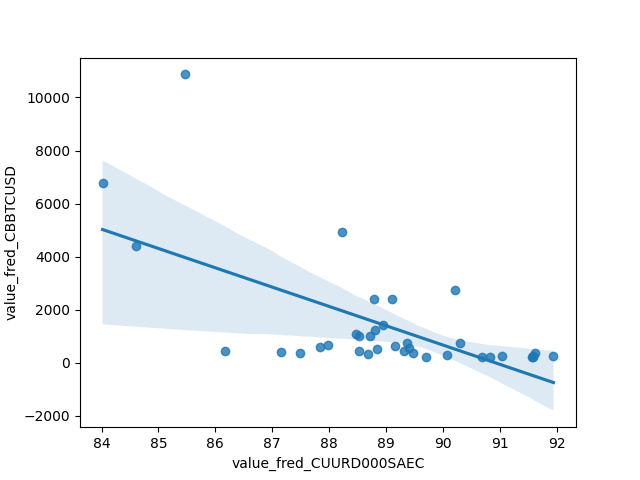
\includegraphics[scale = 0.9]{plots/plot_2024-10-06.png}
\caption{Regression Plot for 2024-10-06}
\end{figure}
\newpage


\end{document}
